\subsection{Continental}
\begin{frame}{L'entreprise Continental}

	\begin{itemize}
		\item Entreprise allemande
			\begin{itemize}
				\item Créée en 1871
				\item Plus de $189\;000$ employés\newline
				$\rightarrow$ Dont $2\;000$ à Toulouse
				\item Dans 50 pays différents
			\end{itemize}

			\begin{figure}[H]
				\only<1>{
					\hspace{-30px}
					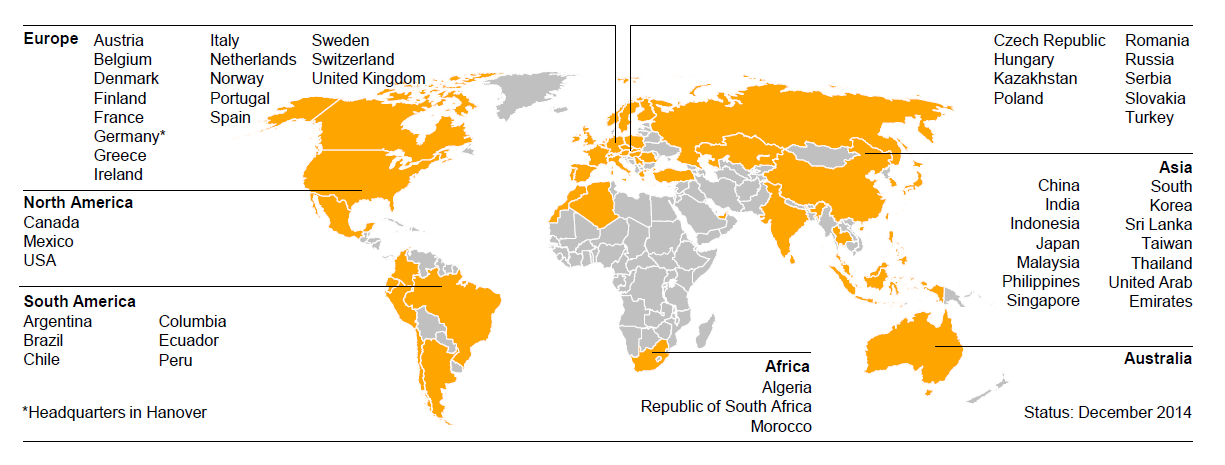
\includegraphics[width=9.5cm]{images/repartition_conti.png}
									\caption{Répartition de Continental dans le monde}
				}
				\only<2>{
					\vspace{-10px}
					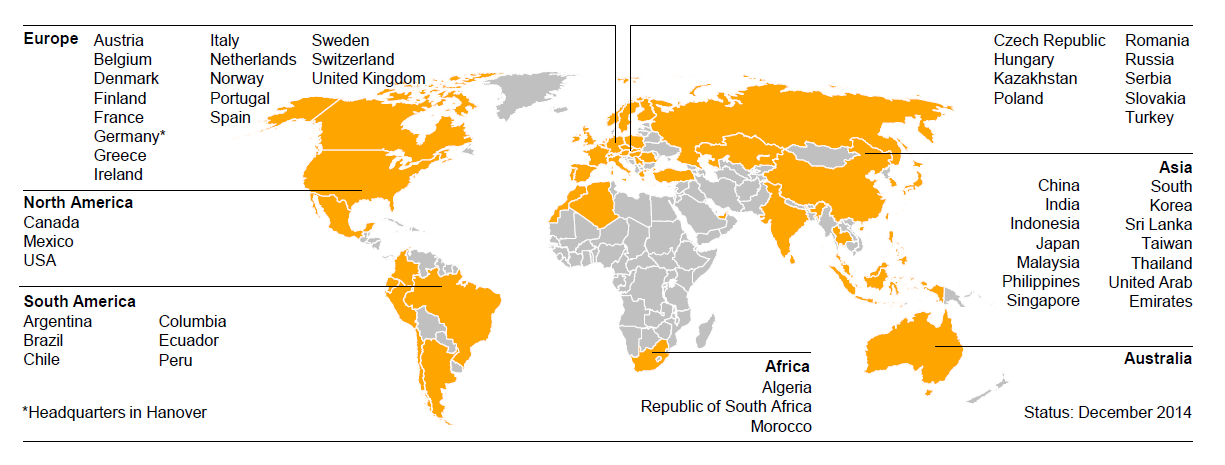
\includegraphics[width=6.5cm]{images/repartition_conti.png}
					\vspace{-10px}
					\caption{\scriptsize Répartition de Continental dans le monde}
				}

			\end{figure}
			\vfill				
		\only<2>{
								\vspace{-10px}
		\item Equipementier Automobile
			\begin{itemize}
				\item Pneus
				\item Sécurité Automobile
				\item Injecteurs
				\item Contrôle moteur
				\item \ldots			
			\end{itemize}
		}
	\end{itemize}
\end{frame}
\subsection{Le groupe Tests Automation Service}
\begin{frame}{Le groupe Tests Automation Service}

	\begin{itemize}
		\item Appartient à la division << \textit{Powertrain} >>
			\begin{itemize}
				\item Calculateurs de contrôle moteur
				\item Mise au point des systèmes essence ou diesel
			\end{itemize}
	\end{itemize}
	
	\vfill
	\pause
	\begin{block}{Le besoin}
		\begin{itemize}
			\item Système à haut risque 
			\item Très complexe
			\begin{itemize}
				\item Des milliers de variables
				\item Des milliers de pages de spécifications
			\end{itemize}
			$\Rightarrow$ Automatisation des tests indispensable
		\end{itemize}
	\end{block}
	\pause
	\begin{itemize}
		\item Le groupe doit fournir des services de tests :
			\begin{itemize}
				\item Tests d'intégration
				\item Tests de non régression
			\end{itemize}
	\end{itemize}
\end{frame}
